\documentclass{article} % For LaTeX2e
\usepackage[T1]{fontenc}
\usepackage{iclr2027_conference,times}

% Optional math commands from https://github.com/goodfeli/dlbook_notation.
%%%%% NEW MATH DEFINITIONS %%%%%

\usepackage{amsmath,amsfonts,bm}

% Mark sections of captions for referring to divisions of figures
\newcommand{\figleft}{{\em (Left)}}
\newcommand{\figcenter}{{\em (Center)}}
\newcommand{\figright}{{\em (Right)}}
\newcommand{\figtop}{{\em (Top)}}
\newcommand{\figbottom}{{\em (Bottom)}}
\newcommand{\captiona}{{\em (a)}}
\newcommand{\captionb}{{\em (b)}}
\newcommand{\captionc}{{\em (c)}}
\newcommand{\captiond}{{\em (d)}}

% Highlight a newly defined term
\newcommand{\newterm}[1]{{\bf #1}}


% Figure reference, lower-case.
\def\figref#1{figure~\ref{#1}}
% Figure reference, capital. For start of sentence
\def\Figref#1{Figure~\ref{#1}}
\def\twofigref#1#2{figures \ref{#1} and \ref{#2}}
\def\quadfigref#1#2#3#4{figures \ref{#1}, \ref{#2}, \ref{#3} and \ref{#4}}
% Section reference, lower-case.
\def\secref#1{section~\ref{#1}}
% Section reference, capital.
\def\Secref#1{Section~\ref{#1}}
% Reference to two sections.
\def\twosecrefs#1#2{sections \ref{#1} and \ref{#2}}
% Reference to three sections.
\def\secrefs#1#2#3{sections \ref{#1}, \ref{#2} and \ref{#3}}
% Reference to an equation, lower-case.
\def\eqref#1{equation~\ref{#1}}
% Reference to an equation, upper case
\def\Eqref#1{Equation~\ref{#1}}
% A raw reference to an equation---avoid using if possible
\def\plaineqref#1{\ref{#1}}
% Reference to a chapter, lower-case.
\def\chapref#1{chapter~\ref{#1}}
% Reference to an equation, upper case.
\def\Chapref#1{Chapter~\ref{#1}}
% Reference to a range of chapters
\def\rangechapref#1#2{chapters\ref{#1}--\ref{#2}}
% Reference to an algorithm, lower-case.
\def\algref#1{algorithm~\ref{#1}}
% Reference to an algorithm, upper case.
\def\Algref#1{Algorithm~\ref{#1}}
\def\twoalgref#1#2{algorithms \ref{#1} and \ref{#2}}
\def\Twoalgref#1#2{Algorithms \ref{#1} and \ref{#2}}
% Reference to a part, lower case
\def\partref#1{part~\ref{#1}}
% Reference to a part, upper case
\def\Partref#1{Part~\ref{#1}}
\def\twopartref#1#2{parts \ref{#1} and \ref{#2}}

\def\ceil#1{\lceil #1 \rceil}
\def\floor#1{\lfloor #1 \rfloor}
\def\1{\bm{1}}
\newcommand{\train}{\mathcal{D}}
\newcommand{\valid}{\mathcal{D_{\mathrm{valid}}}}
\newcommand{\test}{\mathcal{D_{\mathrm{test}}}}

\def\eps{{\epsilon}}


% Random variables
\def\reta{{\textnormal{$\eta$}}}
\def\ra{{\textnormal{a}}}
\def\rb{{\textnormal{b}}}
\def\rc{{\textnormal{c}}}
\def\rd{{\textnormal{d}}}
\def\re{{\textnormal{e}}}
\def\rf{{\textnormal{f}}}
\def\rg{{\textnormal{g}}}
\def\rh{{\textnormal{h}}}
\def\ri{{\textnormal{i}}}
\def\rj{{\textnormal{j}}}
\def\rk{{\textnormal{k}}}
\def\rl{{\textnormal{l}}}
% rm is already a command, just don't name any random variables m
\def\rn{{\textnormal{n}}}
\def\ro{{\textnormal{o}}}
\def\rp{{\textnormal{p}}}
\def\rq{{\textnormal{q}}}
\def\rr{{\textnormal{r}}}
\def\rs{{\textnormal{s}}}
\def\rt{{\textnormal{t}}}
\def\ru{{\textnormal{u}}}
\def\rv{{\textnormal{v}}}
\def\rw{{\textnormal{w}}}
\def\rx{{\textnormal{x}}}
\def\ry{{\textnormal{y}}}
\def\rz{{\textnormal{z}}}

% Random vectors
\def\rvepsilon{{\mathbf{\epsilon}}}
\def\rvtheta{{\mathbf{\theta}}}
\def\rva{{\mathbf{a}}}
\def\rvb{{\mathbf{b}}}
\def\rvc{{\mathbf{c}}}
\def\rvd{{\mathbf{d}}}
\def\rve{{\mathbf{e}}}
\def\rvf{{\mathbf{f}}}
\def\rvg{{\mathbf{g}}}
\def\rvh{{\mathbf{h}}}
\def\rvu{{\mathbf{i}}}
\def\rvj{{\mathbf{j}}}
\def\rvk{{\mathbf{k}}}
\def\rvl{{\mathbf{l}}}
\def\rvm{{\mathbf{m}}}
\def\rvn{{\mathbf{n}}}
\def\rvo{{\mathbf{o}}}
\def\rvp{{\mathbf{p}}}
\def\rvq{{\mathbf{q}}}
\def\rvr{{\mathbf{r}}}
\def\rvs{{\mathbf{s}}}
\def\rvt{{\mathbf{t}}}
\def\rvu{{\mathbf{u}}}
\def\rvv{{\mathbf{v}}}
\def\rvw{{\mathbf{w}}}
\def\rvx{{\mathbf{x}}}
\def\rvy{{\mathbf{y}}}
\def\rvz{{\mathbf{z}}}

% Elements of random vectors
\def\erva{{\textnormal{a}}}
\def\ervb{{\textnormal{b}}}
\def\ervc{{\textnormal{c}}}
\def\ervd{{\textnormal{d}}}
\def\erve{{\textnormal{e}}}
\def\ervf{{\textnormal{f}}}
\def\ervg{{\textnormal{g}}}
\def\ervh{{\textnormal{h}}}
\def\ervi{{\textnormal{i}}}
\def\ervj{{\textnormal{j}}}
\def\ervk{{\textnormal{k}}}
\def\ervl{{\textnormal{l}}}
\def\ervm{{\textnormal{m}}}
\def\ervn{{\textnormal{n}}}
\def\ervo{{\textnormal{o}}}
\def\ervp{{\textnormal{p}}}
\def\ervq{{\textnormal{q}}}
\def\ervr{{\textnormal{r}}}
\def\ervs{{\textnormal{s}}}
\def\ervt{{\textnormal{t}}}
\def\ervu{{\textnormal{u}}}
\def\ervv{{\textnormal{v}}}
\def\ervw{{\textnormal{w}}}
\def\ervx{{\textnormal{x}}}
\def\ervy{{\textnormal{y}}}
\def\ervz{{\textnormal{z}}}

% Random matrices
\def\rmA{{\mathbf{A}}}
\def\rmB{{\mathbf{B}}}
\def\rmC{{\mathbf{C}}}
\def\rmD{{\mathbf{D}}}
\def\rmE{{\mathbf{E}}}
\def\rmF{{\mathbf{F}}}
\def\rmG{{\mathbf{G}}}
\def\rmH{{\mathbf{H}}}
\def\rmI{{\mathbf{I}}}
\def\rmJ{{\mathbf{J}}}
\def\rmK{{\mathbf{K}}}
\def\rmL{{\mathbf{L}}}
\def\rmM{{\mathbf{M}}}
\def\rmN{{\mathbf{N}}}
\def\rmO{{\mathbf{O}}}
\def\rmP{{\mathbf{P}}}
\def\rmQ{{\mathbf{Q}}}
\def\rmR{{\mathbf{R}}}
\def\rmS{{\mathbf{S}}}
\def\rmT{{\mathbf{T}}}
\def\rmU{{\mathbf{U}}}
\def\rmV{{\mathbf{V}}}
\def\rmW{{\mathbf{W}}}
\def\rmX{{\mathbf{X}}}
\def\rmY{{\mathbf{Y}}}
\def\rmZ{{\mathbf{Z}}}

% Elements of random matrices
\def\ermA{{\textnormal{A}}}
\def\ermB{{\textnormal{B}}}
\def\ermC{{\textnormal{C}}}
\def\ermD{{\textnormal{D}}}
\def\ermE{{\textnormal{E}}}
\def\ermF{{\textnormal{F}}}
\def\ermG{{\textnormal{G}}}
\def\ermH{{\textnormal{H}}}
\def\ermI{{\textnormal{I}}}
\def\ermJ{{\textnormal{J}}}
\def\ermK{{\textnormal{K}}}
\def\ermL{{\textnormal{L}}}
\def\ermM{{\textnormal{M}}}
\def\ermN{{\textnormal{N}}}
\def\ermO{{\textnormal{O}}}
\def\ermP{{\textnormal{P}}}
\def\ermQ{{\textnormal{Q}}}
\def\ermR{{\textnormal{R}}}
\def\ermS{{\textnormal{S}}}
\def\ermT{{\textnormal{T}}}
\def\ermU{{\textnormal{U}}}
\def\ermV{{\textnormal{V}}}
\def\ermW{{\textnormal{W}}}
\def\ermX{{\textnormal{X}}}
\def\ermY{{\textnormal{Y}}}
\def\ermZ{{\textnormal{Z}}}

% Vectors
\def\vzero{{\bm{0}}}
\def\vone{{\bm{1}}}
\def\vmu{{\bm{\mu}}}
\def\vtheta{{\bm{\theta}}}
\def\va{{\bm{a}}}
\def\vb{{\bm{b}}}
\def\vc{{\bm{c}}}
\def\vd{{\bm{d}}}
\def\ve{{\bm{e}}}
\def\vf{{\bm{f}}}
\def\vg{{\bm{g}}}
\def\vh{{\bm{h}}}
\def\vi{{\bm{i}}}
\def\vj{{\bm{j}}}
\def\vk{{\bm{k}}}
\def\vl{{\bm{l}}}
\def\vm{{\bm{m}}}
\def\vn{{\bm{n}}}
\def\vo{{\bm{o}}}
\def\vp{{\bm{p}}}
\def\vq{{\bm{q}}}
\def\vr{{\bm{r}}}
\def\vs{{\bm{s}}}
\def\vt{{\bm{t}}}
\def\vu{{\bm{u}}}
\def\vv{{\bm{v}}}
\def\vw{{\bm{w}}}
\def\vx{{\bm{x}}}
\def\vy{{\bm{y}}}
\def\vz{{\bm{z}}}

% Elements of vectors
\def\evalpha{{\alpha}}
\def\evbeta{{\beta}}
\def\evepsilon{{\epsilon}}
\def\evlambda{{\lambda}}
\def\evomega{{\omega}}
\def\evmu{{\mu}}
\def\evpsi{{\psi}}
\def\evsigma{{\sigma}}
\def\evtheta{{\theta}}
\def\eva{{a}}
\def\evb{{b}}
\def\evc{{c}}
\def\evd{{d}}
\def\eve{{e}}
\def\evf{{f}}
\def\evg{{g}}
\def\evh{{h}}
\def\evi{{i}}
\def\evj{{j}}
\def\evk{{k}}
\def\evl{{l}}
\def\evm{{m}}
\def\evn{{n}}
\def\evo{{o}}
\def\evp{{p}}
\def\evq{{q}}
\def\evr{{r}}
\def\evs{{s}}
\def\evt{{t}}
\def\evu{{u}}
\def\evv{{v}}
\def\evw{{w}}
\def\evx{{x}}
\def\evy{{y}}
\def\evz{{z}}

% Matrix
\def\mA{{\bm{A}}}
\def\mB{{\bm{B}}}
\def\mC{{\bm{C}}}
\def\mD{{\bm{D}}}
\def\mE{{\bm{E}}}
\def\mF{{\bm{F}}}
\def\mG{{\bm{G}}}
\def\mH{{\bm{H}}}
\def\mI{{\bm{I}}}
\def\mJ{{\bm{J}}}
\def\mK{{\bm{K}}}
\def\mL{{\bm{L}}}
\def\mM{{\bm{M}}}
\def\mN{{\bm{N}}}
\def\mO{{\bm{O}}}
\def\mP{{\bm{P}}}
\def\mQ{{\bm{Q}}}
\def\mR{{\bm{R}}}
\def\mS{{\bm{S}}}
\def\mT{{\bm{T}}}
\def\mU{{\bm{U}}}
\def\mV{{\bm{V}}}
\def\mW{{\bm{W}}}
\def\mX{{\bm{X}}}
\def\mY{{\bm{Y}}}
\def\mZ{{\bm{Z}}}
\def\mBeta{{\bm{\beta}}}
\def\mPhi{{\bm{\Phi}}}
\def\mLambda{{\bm{\Lambda}}}
\def\mSigma{{\bm{\Sigma}}}

% Tensor
\DeclareMathAlphabet{\mathsfit}{\encodingdefault}{\sfdefault}{m}{sl}
\SetMathAlphabet{\mathsfit}{bold}{\encodingdefault}{\sfdefault}{bx}{n}
\newcommand{\tens}[1]{\bm{\mathsfit{#1}}}
\def\tA{{\tens{A}}}
\def\tB{{\tens{B}}}
\def\tC{{\tens{C}}}
\def\tD{{\tens{D}}}
\def\tE{{\tens{E}}}
\def\tF{{\tens{F}}}
\def\tG{{\tens{G}}}
\def\tH{{\tens{H}}}
\def\tI{{\tens{I}}}
\def\tJ{{\tens{J}}}
\def\tK{{\tens{K}}}
\def\tL{{\tens{L}}}
\def\tM{{\tens{M}}}
\def\tN{{\tens{N}}}
\def\tO{{\tens{O}}}
\def\tP{{\tens{P}}}
\def\tQ{{\tens{Q}}}
\def\tR{{\tens{R}}}
\def\tS{{\tens{S}}}
\def\tT{{\tens{T}}}
\def\tU{{\tens{U}}}
\def\tV{{\tens{V}}}
\def\tW{{\tens{W}}}
\def\tX{{\tens{X}}}
\def\tY{{\tens{Y}}}
\def\tZ{{\tens{Z}}}


% Graph
\def\gA{{\mathcal{A}}}
\def\gB{{\mathcal{B}}}
\def\gC{{\mathcal{C}}}
\def\gD{{\mathcal{D}}}
\def\gE{{\mathcal{E}}}
\def\gF{{\mathcal{F}}}
\def\gG{{\mathcal{G}}}
\def\gH{{\mathcal{H}}}
\def\gI{{\mathcal{I}}}
\def\gJ{{\mathcal{J}}}
\def\gK{{\mathcal{K}}}
\def\gL{{\mathcal{L}}}
\def\gM{{\mathcal{M}}}
\def\gN{{\mathcal{N}}}
\def\gO{{\mathcal{O}}}
\def\gP{{\mathcal{P}}}
\def\gQ{{\mathcal{Q}}}
\def\gR{{\mathcal{R}}}
\def\gS{{\mathcal{S}}}
\def\gT{{\mathcal{T}}}
\def\gU{{\mathcal{U}}}
\def\gV{{\mathcal{V}}}
\def\gW{{\mathcal{W}}}
\def\gX{{\mathcal{X}}}
\def\gY{{\mathcal{Y}}}
\def\gZ{{\mathcal{Z}}}

% Sets
\def\sA{{\mathbb{A}}}
\def\sB{{\mathbb{B}}}
\def\sC{{\mathbb{C}}}
\def\sD{{\mathbb{D}}}
% Don't use a set called E, because this would be the same as our symbol
% for expectation.
\def\sF{{\mathbb{F}}}
\def\sG{{\mathbb{G}}}
\def\sH{{\mathbb{H}}}
\def\sI{{\mathbb{I}}}
\def\sJ{{\mathbb{J}}}
\def\sK{{\mathbb{K}}}
\def\sL{{\mathbb{L}}}
\def\sM{{\mathbb{M}}}
\def\sN{{\mathbb{N}}}
\def\sO{{\mathbb{O}}}
\def\sP{{\mathbb{P}}}
\def\sQ{{\mathbb{Q}}}
\def\sR{{\mathbb{R}}}
\def\sS{{\mathbb{S}}}
\def\sT{{\mathbb{T}}}
\def\sU{{\mathbb{U}}}
\def\sV{{\mathbb{V}}}
\def\sW{{\mathbb{W}}}
\def\sX{{\mathbb{X}}}
\def\sY{{\mathbb{Y}}}
\def\sZ{{\mathbb{Z}}}

% Entries of a matrix
\def\emLambda{{\Lambda}}
\def\emA{{A}}
\def\emB{{B}}
\def\emC{{C}}
\def\emD{{D}}
\def\emE{{E}}
\def\emF{{F}}
\def\emG{{G}}
\def\emH{{H}}
\def\emI{{I}}
\def\emJ{{J}}
\def\emK{{K}}
\def\emL{{L}}
\def\emM{{M}}
\def\emN{{N}}
\def\emO{{O}}
\def\emP{{P}}
\def\emQ{{Q}}
\def\emR{{R}}
\def\emS{{S}}
\def\emT{{T}}
\def\emU{{U}}
\def\emV{{V}}
\def\emW{{W}}
\def\emX{{X}}
\def\emY{{Y}}
\def\emZ{{Z}}
\def\emSigma{{\Sigma}}

% entries of a tensor
% Same font as tensor, without \bm wrapper
\newcommand{\etens}[1]{\mathsfit{#1}}
\def\etLambda{{\etens{\Lambda}}}
\def\etA{{\etens{A}}}
\def\etB{{\etens{B}}}
\def\etC{{\etens{C}}}
\def\etD{{\etens{D}}}
\def\etE{{\etens{E}}}
\def\etF{{\etens{F}}}
\def\etG{{\etens{G}}}
\def\etH{{\etens{H}}}
\def\etI{{\etens{I}}}
\def\etJ{{\etens{J}}}
\def\etK{{\etens{K}}}
\def\etL{{\etens{L}}}
\def\etM{{\etens{M}}}
\def\etN{{\etens{N}}}
\def\etO{{\etens{O}}}
\def\etP{{\etens{P}}}
\def\etQ{{\etens{Q}}}
\def\etR{{\etens{R}}}
\def\etS{{\etens{S}}}
\def\etT{{\etens{T}}}
\def\etU{{\etens{U}}}
\def\etV{{\etens{V}}}
\def\etW{{\etens{W}}}
\def\etX{{\etens{X}}}
\def\etY{{\etens{Y}}}
\def\etZ{{\etens{Z}}}

% The true underlying data generating distribution
\newcommand{\pdata}{p_{\rm{data}}}
% The empirical distribution defined by the training set
\newcommand{\ptrain}{\hat{p}_{\rm{data}}}
\newcommand{\Ptrain}{\hat{P}_{\rm{data}}}
% The model distribution
\newcommand{\pmodel}{p_{\rm{model}}}
\newcommand{\Pmodel}{P_{\rm{model}}}
\newcommand{\ptildemodel}{\tilde{p}_{\rm{model}}}
% Stochastic autoencoder distributions
\newcommand{\pencode}{p_{\rm{encoder}}}
\newcommand{\pdecode}{p_{\rm{decoder}}}
\newcommand{\precons}{p_{\rm{reconstruct}}}

\newcommand{\laplace}{\mathrm{Laplace}} % Laplace distribution

\newcommand{\E}{\mathbb{E}}
\newcommand{\Ls}{\mathcal{L}}
\newcommand{\R}{\mathbb{R}}
\newcommand{\emp}{\tilde{p}}
\newcommand{\lr}{\alpha}
\newcommand{\reg}{\lambda}
\newcommand{\rect}{\mathrm{rectifier}}
\newcommand{\softmax}{\mathrm{softmax}}
\newcommand{\sigmoid}{\sigma}
\newcommand{\softplus}{\zeta}
\newcommand{\KL}{D_{\mathrm{KL}}}
\newcommand{\Var}{\mathrm{Var}}
\newcommand{\standarderror}{\mathrm{SE}}
\newcommand{\Cov}{\mathrm{Cov}}
% Wolfram Mathworld says $L^2$ is for function spaces and $\ell^2$ is for vectors
% But then they seem to use $L^2$ for vectors throughout the site, and so does
% wikipedia.
\newcommand{\normlzero}{L^0}
\newcommand{\normlone}{L^1}
\newcommand{\normltwo}{L^2}
\newcommand{\normlp}{L^p}
\newcommand{\normmax}{L^\infty}

\newcommand{\parents}{Pa} % See usage in notation.tex. Chosen to match Daphne's book.

\DeclareMathOperator*{\argmax}{arg\,max}
\DeclareMathOperator*{\argmin}{arg\,min}

\DeclareMathOperator{\sign}{sign}
\DeclareMathOperator{\Tr}{Tr}
\let\ab\allowbreak


\usepackage{float}
\usepackage{hyperref}
\hypersetup{hidelinks}
\usepackage{url}
\usepackage{booktabs}
\usepackage{graphicx}
\usepackage{array}
\usepackage{xcolor}
\usepackage{tikz}
\usetikzlibrary{arrows.meta,positioning,calc}
\usepackage{enumitem}
\setlist{nosep,leftmargin=*}

\newcommand{\accept}{\textsc{accept}}
\newcommand{\reject}{\textsc{reject}}
\newcommand{\dvv}{DrawVerify}

\title{DrawVerify: Validating Sketched \\ Robot Instructions Before Execution}

<<<<<<< HEAD
=======
% TODO: replace the placeholder names/e-mails below with the team members' details.
>>>>>>> ecbd1642964bb14f56056f5253e72595e899af45
\author{Duc Anh Do, Tran Huu Loc \& Nhat Minh Nguyen \thanks{CS707 Group Project Proposal, Track~B (novel task formulation).} \\
School of Computing and Information Systems \\
Singapore Management University \\
\texttt{\{doducanh.2026, tranhuuloc.2026, nm.nguyen.2026\}@phdcs.smu.edu.sg}
}

\iclrfinalcopy % show author block (course submission, not anonymous)

\begin{document}

\maketitle
\lhead{CS707 Group Project Proposal (ICLR 2027 format) --- Track B}

\begin{abstract}
Circle-and-arrow sketches tell a robot \emph{which} object to move and \emph{where} without naming anything, but existing sketch-conditioned systems execute the drawing unchecked. We study \textbf{sketch-prompt validation}---deciding \emph{before} any action whether a drawn instruction is correct, consistent across circle, arrow, and caption, and sufficient for a unique action, and saying why not---as an explicit pre-execution gate. A pilot by team members built a simulator-grounded generator over LIBERO (8,522 labelled prompts), collected 275 human sketches, and ran a 17-participant in-the-loop study: generated prompts rank validators like human sketches do but inflate AUROC by $+0.13$; a LoRA-adapted Qwen3-VL-4B staged over 82 human sketches reaches 0.808 AUROC, on par with 4-shot Gemini-3.8-Flash; yet live gating gave no detectable improvement, with in-loop precision 0.38 and no diagnostic in the rejection. We propose to (H1) match generated strokes to human statistics and audit geometry-only ceilings, (H2) \emph{generate} a per-channel verdict and rejection reason, (H3) calibrate the operating point with a conformal false-accept guarantee, and (H4) test channel-naming feedback and a one-retry cap in a follow-up study.
\end{abstract}

\section{Problem and Motivation}
\label{sec:problem}

Language is ambiguous in cluttered scenes with duplicate objects and goal images are over-specified \citep{sundaresan2024rtsketch}; a circle-and-arrow sketch with a name-free caption (``move this there'') is a persistent deictic act \citep{sauppe2014deictics,kranstedt2006deixis}. Recent systems condition robot policies on such sketches \citep{sundaresan2024rtsketch,gu2024rttrajectory,li2025crayonrobo,li2025rovi} and all silently assume the drawing is \emph{valid}. Yet circles miss or enclose a distractor, arrows point to the wrong container or detach from the circle, captions contradict sketches, and channels that look fine alone can jointly disagree; executing such a sketch commits the robot to a wrong action.

\begin{figure}[b]
\centering
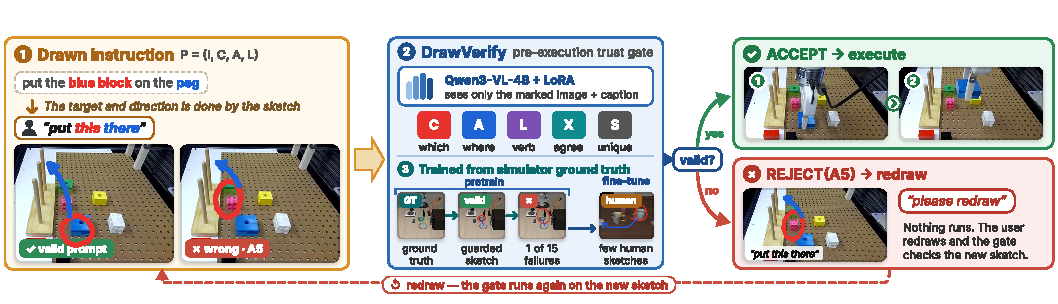
\includegraphics[width=0.6\textwidth]{figures/fig_overview.pdf}
\caption{The pilot validator as a pre-execution trust gate \citep{drawverify2026pilot}: a LoRA-adapted VLM trained on simulator ground truth judges the marked image and caption; \accept{} executes, \reject{} asks the user to redraw.}
\label{fig:overview}
\end{figure}

\textbf{Problem (Track B).} \emph{Can a model decide, before any action, whether a drawn instruction is safe to execute---and say why not?} We formulate \textbf{sketch-prompt validation} as a decision over image, circle, arrow, and caption requiring per-channel correctness, cross-channel consistency, and sufficiency (\Secref{sec:formulation}), plus a generated reason; no existing task captures it (\Secref{sec:related}). We address it with generative VLMs as prompted judges and as LoRA-tuned validators (\Figref{fig:overview}).

\textbf{Pilot evidence and gap.} A pilot by team members \citep{drawverify2026pilot} built \dvv, a simulator-grounded generator over LIBERO \citep{liu2023libero}: 8,522 labelled prompts (31.8\% valid) from 800 demonstrations over 40 tasks, 15 of 18 corruption modes plus five grounding configurations, 275 human sketches (82 train / 193 test), and 326 sketches from a 17-participant in-the-loop study. Findings (Appendix~\ref{app:details}, \Figref{fig:evalsets}): (i)~generated prompts order seven API validators as human sketches do (Spearman $\rho=+0.93$) but inflate AUROC unevenly ($+0.13$ mean, $-0.06$ to $+0.25$); (ii)~Qwen3-VL-4B \citep{qwen3vl2025} with LoRA \citep{hu2022lora} trained on generated prompts alone transfers poorly (0.565 AUROC on human sketches) but staged over 82 human sketches reaches 0.808, matching 4-shot Gemini-3.8-Flash (0.857, n.s.); (iii)~live gating gave \emph{no detectable improvement}: in-loop precision 0.382, third attempts broke more than they repaired, and the rejection carried no diagnostic. The pilot never measured the human-likeness of generated strokes, never tested a per-channel verdict, set its threshold ad hoc, and ran one gated arm without feedback. This project delivers those deltas.

\textbf{Hypotheses.} \textbf{H1 (hardening and transfer):} trained on the hardened tier alone, the validator reaches $\ge$0.70 AUROC on the 193 human test sketches (v1-only: 0.565), while a geometry-only classifier on that tier stays $\le$0.60 AUROC on an untouched audit split. \textbf{H2 (structured supervision):} supervising the five predicates as auxiliary generative targets lifts recall on directional failures of the human test split from 0.53 to $\ge$0.70 at no loss in $R_{\mathrm{val}}$, and generated reasons name the violated predicate with $\ge$80\% faithfulness on generated negatives and $\ge$70\% on human ones. \textbf{H3 (calibrated gate):} with $\hat\tau$ from Eq.~(\ref{eq:crc}), false-accept rate (FAR) on held-out human sketches is $\le\alpha=0.10$ in every seed, and at the pilot's recall (0.786) precision on ungated study sketches beats its 0.458 by $\ge$10 points. \textbf{H4 (feedback):} in a follow-up study ($\ge$20 participants), a gate that names the failing channel under a one-retry cap raises the validity of the finally sent instruction over the bare gate (pilot: 0.795) by $\ge$17 points, the pilot's minimum detectable effect.

\section{Related Work}
\label{sec:related}

\textbf{Sketch- and visual-prompt-based instruction.} RT-Sketch and RT-Trajectory condition policies on goal or trajectory sketches \citep{sundaresan2024rtsketch,gu2024rttrajectory}, RoVI decodes an arrow/circle language with a VLM \citep{li2025rovi}, CrayonRobo \emph{tolerates} noisy prompts but does not classify them \citep{li2025crayonrobo}, and Action-Sketcher, AnyUser and visual-prompting methods \citep{tan2026actionsketcher,yang2026anyuser,nasiriany2024pivot,yang2023som,liu2024moka,yuan2024robopoint,cai2024vipllava} translate or annotate sketches for a VLM. All assume the prompt is valid; \emph{we extend} them by making validity the primary decision.

\textbf{Verification and safety gating.} KnowNo asks for help via conformal prediction \citep{ren2023knowno}; VerifyLLM and VeriGraph verify plans against temporal logic or scene graphs \citep{sautenkov2025verifyllm,ekpo2024verigraph}; DoReMi and REFLECT detect or explain execution failures \citep{guo2024doremi,liu2023reflect}. These verify \emph{plans} or \emph{executions}; \emph{we contrast} by verifying the instruction itself, an earlier gate, with a conformal threshold \citep{angelopoulos2024conformalrisk,geifman2017selective}. Shortcut audits \citep{gururangan2018artifacts,geirhos2020shortcut,swayamdipta2020cartography} filter fixed datasets; \emph{we control the generator}.

\section{Task Formulation and Method Sketch}
\label{sec:method}

\subsection{Formulation}
\label{sec:formulation}
A sketch prompt is $P=(I,C,A,L)$: RGB observation $I$, circle $C$ (centre, radius) denoting \emph{which} object, arrow $A$ (tail, head) denoting \emph{where} it goes, and a name-free caption $L$. From simulator ground truth we define predicates $v_C$ (the circle uniquely selects the target), $v_A$ (correct bearing and magnitude, anchored on the circled object, ending in the intended region), $v_L$ (caption verb and implicit referents match the action), cross-modal consistency $v_X$ (all channels describe the same object, destination, and predicate), and sufficiency $v_S$ (a unique executable action). A prompt is valid iff $V(P)=v_C(P)\wedge v_A(P)\wedge v_L(P)\wedge v_X(P)\wedge v_S(P)$; the task is to learn $f_\theta(P)\in\{\accept,\reject\}$ predicting $V(P)$, with a reason on \reject. A prompt can pass every per-channel predicate yet fail $v_X$ or $v_S$, so validation is not a set of independent checks.

\subsection{Simulator-grounded data generation and shortcut hardening}
\label{sec:data}
\textbf{Pilot pipeline (\Figref{fig:overview}; Appendix \Figref{fig:method}, top).} From LIBERO's object poses, region geometry, and gripper trajectories we extract the correct circle target and arrow endpoints for every frame with no human labelling. Valid prompts get \emph{guarded} human-imprecision augmentation (jitter, non-circular strokes, hand-like shafts), with in-point/out-point guards keeping the target inside the circle and distractors outside. Negatives apply one controlled corruption from four families (15 of 18 modes; Appendix~\ref{app:taxonomy}) plus five grounding configurations, so every negative has a known mode, severity, and violated predicate.

\textbf{New: shortcut hardening (H1).} Let $g(P)$ be the raw geometry vector (circle centre, radius, eccentricity; arrow endpoints, length, bearing, tail offset). (i)~\emph{Distribution matching to humans}: the pilot never compared generated and human strokes; we estimate the marginals of $g$ on the 82 human training sketches and importance-re-sample valid imprecision and corruption severities to match them as far as labels allow, guard-crossing modes (near-miss, wrong magnitude) drawing severities from the mirrored distribution just beyond the guard. (ii)~\emph{Adversarial filtering} \citep{lebras2020aflite} on medium/hard modes: we repeatedly train geometry-only gradient-boosted classifiers \citep{ke2017lightgbm} on random folds and remove the examples held-out classifiers predict most confidently until geometry-only AUROC on an \emph{untouched} audit split is $\le0.60$ or retention falls below 60\%. We also report a \emph{scene-blind} ceiling (sketches on a blank canvas).

\subsection{Structured validator and conformal inference}
\label{sec:validator}
\textbf{Model.} Qwen3-VL-4B (and 2B) with LoRA (rank 32, as in the pilot) takes the image with the rendered sketch, the caption, and a fixed prompt and generates a \emph{structured verdict}: five predicate questions $q_k$, $k\in\{C,A,L,X,S\}$, answered sequentially with earlier answers in context (teacher-forced in training), then the \accept/\reject{} question $q_V$, then, on \reject, a one-sentence reason naming the failing channel. Training keeps the pilot's staged recipe (generated tier, then the 82 human sketches). Predicate labels are free: each generated negative violates a known subset and human negatives carry an annotator failure code.

\textbf{Objective.} Each yes/no answer is scored by forced choice over its two answer tokens, $p_\theta(\text{yes}\mid P,q_k)=\sigma(z_{\text{yes}}-z_{\text{no}})$; the reason uses token-level cross-entropy $\ell_R$ on \reject{} examples against paraphrased template reasons per mode. We minimise
\begin{equation}
\mathcal{L}(\theta)=\ell_V(\theta)+\lambda\!\!\sum_{k\in\{C,A,L,X,S\}}\!\!\ell_k(\theta)+\mu\,\ell_R(\theta),\qquad
\ell_k(\theta)=-\log p_\theta\big(y_k \mid P, q_k\big),
\label{eq:loss}
\end{equation}
with $\lambda,\mu$ tuned on validation; $\lambda=\mu=0$ recovers the pilot's answer-only validator (ablation A1).

\textbf{Inference with a finite-sample false-accept guarantee.} Let $s(P)=p_\theta(\accept\mid P,q_V)$, read from the \textsc{valid}/\textsc{wrong} token probabilities as in the pilot; we \accept{} iff $s(P)\ge\hat\tau$. False accepts are the safety-critical error, so we bound their rate by conformal risk control \citep{angelopoulos2024conformalrisk}: on the $n$ \emph{invalid} calibration sketches let $\ell_i(\tau)=\mathbb{1}[s(P_i)\ge\tau]$ and
\begin{equation}
\hat\tau=\inf\big\{\tau:\ \tfrac{1}{n+1}\textstyle\sum_{i=1}^{n}\ell_i(\tau)+\tfrac{1}{n+1}\le\alpha\big\}.
\label{eq:crc}
\end{equation}
If calibration and test prompts are exchangeable, $\mathbb{E}[\mathrm{FAR}(\hat\tau)]\le\alpha$; with $n\approx35$ invalid calibration sketches $\alpha\ge1/(n{+}1)$, hence $\alpha=0.10$. We report the induced false-reject rate, precision at matched recall, and coverage across seeds, tiers, and study sketches (where exchangeability is \emph{not} guaranteed).

\section{Datasets, Metrics, Baselines, and Experimental Plan}
\label{sec:plan}

\textbf{Datasets and licences.} (1)~\emph{LIBERO} \citep{liu2023libero} (MIT): 800 demonstrations, 40 tasks. (2)~\emph{\dvv{} v1} (pilot): 8,522 prompts---6,463 / 900 / 1,159 train / val / test, demo-disjoint, 68.2\% invalid (Appendix~\ref{app:taxonomy})---with image, coordinates, caption, label, and mode. (3)~\emph{v2 (hardened)}: same splits after matching and filtering ($\ge$60\% retention expected) plus the untouched audit split. (4)~\emph{Human sketches} (pilot; Appendix~\ref{app:details}): the 275-sketch corpus (157 valid / 118 invalid, task-disjoint 82 train / 193 test, annotator failure codes) and the 326 study sketches (88 ungated); the 82 training sketches double as calibration set. (5)~\emph{Follow-up study} (new; IRB exemption first): $\ge$20 adult volunteers, 21 trials each in three counterbalanced blocks (bare gate; channel-naming gate; with one-retry cap), with the pilot's interface and blind labelling deck. Data and adapters: CC~BY~4.0; code: MIT.

\textbf{Metrics.} AUROC (invalid as positive class), accuracy, precision and recall on invalid prompts, $R_{\mathrm{val}}$ (recall on valid), MCC; FAR, FRR and precision at $\hat\tau$; recall per failure family and mode; geometry-only and scene-blind ceilings per tier; ranking agreement $\rho$ with human sets; reason faithfulness against the ground-truth predicate or annotator failure code (string match, Qwen3-8B judge); study outcomes as in the pilot: validity of the finally sent instruction, attempts per trial, fix/break counts (Wilson intervals).

\textbf{Baselines.} (i)~Majority class. (ii)~The pilot's seven API models (Gemini-3.8-Flash, GPT-5-mini, GPT-4.1-mini, Gemini-2.5-Flash, Claude-Haiku-4.5, GPT-5-nano, Claude-3-Haiku) under the identical 4-shot prompt, cached outputs reused. (iii)~Zero-shot Qwen3-VL-2B/4B. (iv)~Geometry-only LightGBM fits and the scene-blind validator as ceilings. (v)~A fine-tuned discriminative model (ConvNeXt-T, late fusion of $g(P)$ and a caption embedding). (vi)~The pilot's staged validators, rationale (0.808 AUROC) and answer-only (0.841). \emph{Ours:} structured validator with the conformal gate.

\textbf{Ablations ($\ge$3), sensitivity, statistics.} A1: structured vs.\ answer-only vs.\ free rationale ($\lambda=\mu=0$; H2). A2: v2 vs.\ v1, with and without the human stage (H1). A3: modality (no caption; coordinates-as-text; scene-blind). A4: no guarded augmentation. A5: calibration set 40 vs.\ 82 and $\alpha\in\{0.05,0.10,0.20\}$ (H3). A6: backbone Qwen3-VL-2B/4B, Qwen2-VL-2B. Sensitivity: training-set size, LoRA rank, corruption severity. 3 seeds (mean$\pm$std); paired bootstrap (2,000 resamples) for AUROC differences, McNemar's test \citep{dietterich1998tests} on seed-matched decisions, Williams' test for dependent $\rho$, minimum detectable effects per slice and for the study.

\section{Risks, Resources, and Team Plan}
\label{sec:risks}
\textbf{Risks and mitigations.} \textbf{Hardening over-removes or still leaks:} per-mode retention curves, removal capped at 40\%, both tiers released. \textbf{Small human sets:} 35 invalid calibration and 82 invalid test sketches; every human-set claim carries bootstrap CIs. \textbf{Study power:} the pilot's minimum detectable effect was 17 points with 12 participants; we recruit $\ge$20, within-participant, and replay logged attempts under the one-retry cap. \textbf{API drift, cost, compute:} pinned versions, cached pilot outputs; $\approx$2 GPU-h per Qwen3-VL-4B run (estimated from the pilot's 2-epoch stage), $\approx$45 runs $\approx$100 GPU-h on one A100/4090, $\approx$USD~100--150 of API calls. \textbf{Schedule:} go/no-go 25 Oct---if the v2 ceiling is still $\ge0.75$ at 60\% retention we report the best partial tier and shift effort to H2--H4. \textbf{Over-claiming safety:} the gate reduces, not eliminates, unsafe executions; nothing is executed on a robot.

\textbf{Roles and timeline (2026).} \emph{Member~1 (data):} generator v2, matching, audit, release. \emph{Member~2 (modelling):} structured objective, reasons, gate, LoRA training, ablations. \emph{Member~3 (evaluation):} API baselines, statistics, follow-up study, ethics. \emph{1--11 Oct:} IRB, recruitment, feedback interface. \emph{12--25 Oct:} generator v2, structured validator and gate, A1--A3; go/no-go. \emph{26 Oct--8 Nov:} follow-up study (H4), A4--A6, statistics. \emph{9--12 Nov:} final presentation ($\ge$90\% of results); \emph{13--27 Nov:} final report and artifacts.

\subsection*{Ethics and reproducibility statements}
Training data are simulator renders with no people or personal data; both sketch studies use consenting adult volunteers and store only drawings, prompts, and anonymous ratings. A false accept could cause a wrong physical action, so we report false-accept rates with confidence intervals and recommend human confirmation at deployment. Licences: LIBERO (MIT), Qwen (Apache-2.0), API terms; we release data and adapters under CC~BY~4.0 and code under MIT, with seeds, cached API outputs, both tiers with checksums, and study and compute logs.

\bibliography{proposal}
\bibliographystyle{iclr2027_conference}

\raggedbottom
\appendix
\section{Failure Taxonomy and Dataset Composition}
\label{app:taxonomy}

\begin{figure}[H]
\centering
\resizebox{0.95\textwidth}{!}{%
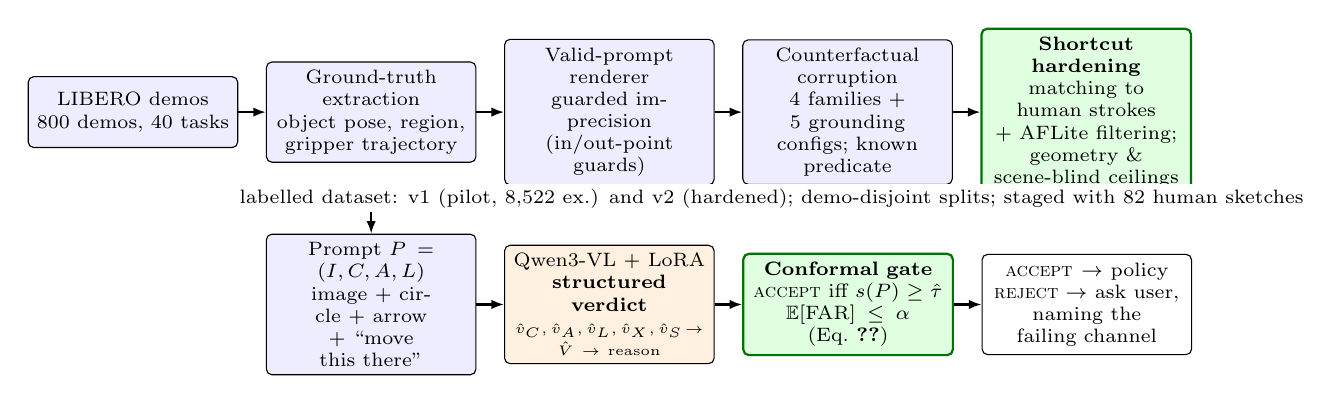
\begin{tikzpicture}[
  font=\scriptsize,
  box/.style={draw, rounded corners=2pt, align=center, minimum height=0.9cm, inner sep=3pt, text width=2.45cm},
  data/.style={box, fill=blue!7},
  model/.style={box, fill=orange!12},
  new/.style={box, fill=green!12, draw=green!45!black, thick},
  arr/.style={-{Latex[length=1.6mm]}, thick},
  node distance=0.45cm and 0.35cm
]
\node[data] (demos) {LIBERO demos\\800 demos, 40 tasks};
\node[data, right=of demos] (gt) {Ground-truth extraction\\object pose, region,\\gripper trajectory};
\node[data, right=of gt] (valid) {Valid-prompt renderer\\guarded imprecision\\(in/out-point guards)};
\node[data, right=of valid] (neg) {Counterfactual corruption\\4 families + 5 grounding\\configs; known predicate};
\node[new, right=of neg] (hard) {\textbf{Shortcut hardening}\\matching to human strokes\\+ AFLite filtering;\\geometry \& scene-blind ceilings};
\draw[arr] (demos) -- (gt); \draw[arr] (gt) -- (valid); \draw[arr] (valid) -- (neg); \draw[arr] (neg) -- (hard);
\node[data, below=0.9cm of gt] (prompt) {Prompt $P=(I,C,A,L)$\\image + circle + arrow\\+ ``move this there''};
\node[model, right=of prompt] (vlm) {Qwen3-VL + LoRA\\\textbf{structured verdict}\\{\tiny $\hat v_C,\hat v_A,\hat v_L,\hat v_X,\hat v_S\!\to\!\hat V\!\to$ reason}};
\node[new, right=of vlm] (gate) {\textbf{Conformal gate}\\$\accept$ iff $s(P)\ge\hat\tau$\\$\mathbb{E}[\mathrm{FAR}]\le\alpha$ (Eq.~\ref{eq:crc})};
\node[box, right=of gate] (out) {$\accept\to$ policy\\$\reject\to$ ask user,\\naming the failing channel};
\draw[arr] (prompt) -- (vlm); \draw[arr] (vlm) -- (gate); \draw[arr] (gate) -- (out);
\draw[arr] (hard.south) |- node[pos=0.72, fill=white, inner sep=1.5pt]{labelled dataset: v1 (pilot, 8,522 ex.) and v2 (hardened); demo-disjoint splits; staged with 82 human sketches} ($(prompt.north)+(0,0.45)$) -- (prompt.north);
\end{tikzpicture}}
\caption{Method sketch (referenced from \Secref{sec:data}). \emph{Top:} simulator-grounded data generation (green = new). \emph{Bottom:} the validator generates a structured verdict and a reason; a conformal threshold yields an execute/ask decision.}
\label{fig:method}
\end{figure}

\begin{table}[H]
\caption{Failure taxonomy of the pilot release. Families A--D define 18 corruption modes, of which 15 are instantiated (Cov.\ \checkmark); C2, D1, D2 are unreachable under name-free captions (N/A) and become reachable in v2 through a named-caption slice. The Grounding family is counted separately. Mode IDs are the generator's keys and are non-contiguous.}
\label{tab:taxonomy}
\begin{center}
\scriptsize
\begin{tabular}{@{}p{2.3cm}lp{7.6cm}c@{}}
\toprule
Family & ID & Mode and generation mechanism & Cov. \\
\midrule
Referential (circle / ``which''; $v_C$) & A2 & Wrong-category object: circle a clearly different object than the target. & \checkmark \\
 & A3 & Near-miss circle: offset the centre so the target falls outside or only grazes the circle. & \checkmark \\
 & A4 & Empty-region circle: circle bare table or background. & \checkmark \\
 & A5 & Multi-object enclosure: inflate the radius to enclose the target and a distractor (tests $v_S$). & \checkmark \\
 & A6 & Degenerate size: dot-sized or whole-frame circle. & \checkmark \\
\midrule
Directional (arrow / ``where''; $v_A$) & B1 & Wrong destination: retarget the head to a different container or region. & \checkmark \\
 & B3 & Wrong magnitude: correct bearing, arrow far too short or overshooting. & \checkmark \\
 & B4 & Wrong bearing: correct length, head rotated $90^\circ$/$180^\circ$. & \checkmark \\
 & B5 & Null destination: head on empty table or off-frame. & \checkmark \\
 & B6 & Detached tail: shaft plausible but tail not anchored on the circled object. & \checkmark \\
 & B7 & Spec mismatch: arrow present on a circle-only task, or missing on a place task. & \checkmark \\
\midrule
Cross-modal ($v_X$) & C1 & Circle--arrow mismatch: circle object A while the arrow originates from object B. & \checkmark \\
 & C2 & Caption--sketch mismatch: correct sketch, caption swapped from another task. & N/A \\
 & C3 & Predicate mismatch: caption says ``open the cabinet'' while the sketch is a place-style circle+arrow. & \checkmark \\
\midrule
Language (caption / ``what''; $v_L$) & D1 & Wrong target noun. & N/A \\
 & D2 & Wrong destination noun. & N/A \\
 & D3 & Wrong verb (pick vs.\ push vs.\ open). & \checkmark \\
 & D4 & Under-determined caption: ``put this there'', valid with a good sketch, invalid with a bad one. & \checkmark \\
\midrule
Grounding ($v_S$) & -- & Five configurations: resolved; no sketch; open destination; twin referents; arrow between destinations. & \checkmark \\
\bottomrule
\end{tabular}
\end{center}
\end{table}

\begin{table}[H]
\caption{\dvv{} v1 composition by label (train / validation / test). Percentages are shares within a split; the label balance is held constant across splits, and no demonstration contributes frames to more than one split.}
\label{tab:composition}
\begin{center}
\small
\begin{tabular}{lrrrr}
\toprule
Label & Train & Val & Test & Total \\
\midrule
Valid & 2,057 (31.8\%) & 285 (31.7\%) & 366 (31.6\%) & 2,708 (31.8\%) \\
Invalid & 4,406 (68.2\%) & 615 (68.3\%) & 793 (68.4\%) & 5,814 (68.2\%) \\
\midrule
Total & 6,463 & 900 & 1,159 & 8,522 \\
\bottomrule
\end{tabular}
\end{center}
\end{table}

\section{Pilot Results, Training Details, and Protocols}
\label{app:details}

\begin{figure}[H]
\centering
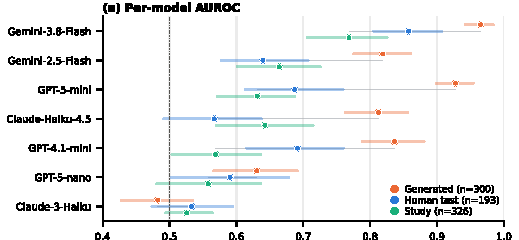
\includegraphics[width=0.55\textwidth]{figures/fig_auroc.pdf}
\caption{Pilot evidence (referenced from \Secref{sec:plan}): AUROC of seven API validators on generated prompts, the human test split and the in-the-loop study (95\% bootstrap intervals). Generated prompts rank models like human sketches do but inflate absolute scores unevenly, motivating H1 and H3.}
\label{fig:evalsets}
\end{figure}

\begin{table}[H]
\caption{Pilot: seven API models under the identical 4-shot prompt on generated prompts (Gen., $n=300$, 60.0\% invalid), the human test split (Test, $n=193$, 42.5\% invalid) and the in-the-loop study (Study, $n=326$, 23.6\% invalid). The last rows give each human set's Spearman agreement with the generated ranking and the fraction of the 21 model pairs whose order is preserved.}
\label{tab:api}
\begin{center}
\small
\begin{tabular}{lcccccc}
\toprule
 & \multicolumn{3}{c}{AUROC} & \multicolumn{3}{c}{MCC} \\
\cmidrule(lr){2-4}\cmidrule(lr){5-7}
Model & Gen. & Test & Study & Gen. & Test & Study \\
\midrule
Gemini-3.8-Flash & \textbf{0.965} & \textbf{0.857} & \textbf{0.768} & $+0.85$ & $+0.50$ & $+0.43$ \\
GPT-5-mini & 0.928 & 0.687 & 0.631 & $+0.82$ & $+0.24$ & $+0.25$ \\
GPT-4.1-mini & 0.836 & 0.691 & 0.569 & $+0.64$ & $+0.24$ & $+0.15$ \\
Gemini-2.5-Flash & 0.818 & 0.640 & 0.664 & $+0.65$ & $+0.29$ & $+0.25$ \\
Claude-Haiku-4.5 & 0.812 & 0.567 & 0.642 & $+0.61$ & $+0.10$ & $+0.27$ \\
GPT-5-nano & 0.630 & 0.591 & 0.558 & $+0.31$ & $+0.26$ & $+0.10$ \\
Claude-3-Haiku & 0.482 & 0.533 & 0.526 & $-0.03$ & $+0.07$ & $+0.10$ \\
\midrule
Mean & 0.782 & 0.652 & 0.623 & $+0.55$ & $+0.24$ & $+0.22$ \\
$\rho$ vs.\ Gen. & & $+0.93$ & $+0.71$ & & $+0.71$ & $+0.75$ \\
Pairs preserved & & 19/21 & 17/21 & & 17/21 & 17/21 \\
\bottomrule
\end{tabular}
\end{center}
\end{table}

\begin{table}[H]
\caption{Pilot: fine-tuned validators against Gemini-3.8-Flash on the human test split ($n=193$, 42.5\% invalid). Positive class is \textsc{invalid}; Prec and Rec are on invalid prompts, $R_{\mathrm{val}}$ is recall on valid ones. $\Delta$ is the paired AUROC difference to Gemini-3.8-Flash, $^*$ marking a 95\% bootstrap interval excluding zero. ``gen$\to$hum'' is the staged recipe; decisions are the generated verdict.}
\label{tab:pilot}
\begin{center}
\footnotesize
\begin{tabular}{lccccccc}
\toprule
Model & Acc & Prec & Rec & MCC & $R_{\mathrm{val}}$ & AUROC & $\Delta$ \\
\midrule
Gemini-3.8-Flash (4-shot) & 0.699 & 0.590 & 0.963 & $+0.50$ & 0.505 & 0.857 & \\
Qwen3-VL-4B zero-shot & 0.585 & 0.600 & 0.073 & $+0.08$ & 0.964 & 0.542 & $-0.32^*$ \\
Qwen3-VL-4B generated only & 0.653 & 0.559 & 0.866 & $+0.38$ & 0.495 & 0.565 & $-0.29^*$ \\
Qwen3-VL-4B human only (82) & 0.627 & 0.561 & 0.561 & $+0.24$ & 0.676 & 0.640 & $-0.22^*$ \\
Qwen3-VL-4B mixed (pooled) & 0.684 & 0.598 & 0.780 & $+0.39$ & 0.613 & 0.754 & $-0.10^*$ \\
Qwen3-VL-4B gen$\to$hum & 0.798 & 0.779 & 0.732 & $+0.58$ & 0.847 & 0.808 & $-0.05$ \\
\quad answer-only & 0.808 & 0.817 & 0.707 & $+0.61$ & 0.883 & 0.841 & $-0.02$ \\
\quad 40 human sketches & 0.782 & 0.900 & 0.549 & $+0.57$ & 0.955 & 0.847 & $-0.01$ \\
Qwen3-VL-2B gen$\to$hum & 0.762 & 0.757 & 0.646 & $+0.51$ & 0.847 & 0.779 & $-0.08^*$ \\
Qwen2-VL-2B gen$\to$hum & 0.741 & 0.767 & 0.561 & $+0.46$ & 0.874 & 0.720 & $-0.14^*$ \\
\midrule
Geometry-only LightGBM (gen.\ fit) & -- & -- & -- & -- & -- & 0.741 & $^*$ \\
\bottomrule
\end{tabular}
\end{center}
\end{table}

\textbf{Fine-tuning (pilot recipe).} LoRA rank 32, $\alpha=64$, dropout 0.05 on the query, key, value and output projections and the gate, up and down MLP projections (0.93\% of Qwen3-VL-4B's parameters). Stage~1: 2 epochs on the generated tier, effective batch 16, learning rate $10^{-4}$ with cosine schedule and 30 warm-up steps (AdamW, no weight decay, gradient clipping 1.0). Stage~2: 4 epochs on the 82 human training sketches, batch 8, learning rate $3\times10^{-5}$. Images $512{\times}512$; loss on the assistant turn only. At inference the model generates its reasoning greedily; the prefix up to \texttt{<answer>} is forced and the decision and AUROC score are read from the relative probabilities of the \textsc{valid}/\textsc{wrong} tokens. Seeds: $0.810\pm0.003$ AUROC for the staged 4B model.

\textbf{API protocol.} The same system prompt, the same four in-context examples drawn from the human training split, temperature 0, and a request for a label and a failure probability $p_{\mathrm{fail}}\in[0,100]$, from which AUROC is computed with invalid as the positive class. Unparsable replies are dropped (6, 4 and 20 for GPT-5-nano on the three sets; none for any other model).

\textbf{Human data.} Ungated corpus: 11 participants, 275 sketches over two rounds covering 34 tasks across the four LIBERO suites; median drawing time 8.2\,s; each sketch labelled valid/invalid by human annotators independently of any model, invalid ones with a failure code from the taxonomy; task-disjoint split 82 train / 193 test. In-the-loop study: 17 participants, 21 trials each in three blocks (no gate, model gate, control gate rejecting on the ground-truth geometry of the original annotation); 250 analysed trials, 326 labelled sketches. Outcomes: validity of the finally sent instruction 0.841 (no gate), 0.795 (model gate, 1.38 attempts/trial), 0.726 (control gate); the model gate's in-loop precision 0.382 and recall 0.500; trials accepted at the second attempt were only repaired (6/0), trials that reached a third broke more than they repaired (6 broken / 2 repaired); of six third-attempt breaks, five changed the prompt rather than the drawing. Replaying the logs with a one-retry cap gives 0.821 (model) and 0.762 (control).

\textbf{Pilot error profile.} On the human test split the staged 4B validator's recall on invalid prompts by family is 0.80 (referential), 0.53 (directional) and 0.77 (cross-modal and grounding) against 0.96 / 0.95 / 1.00 for Gemini-3.8-Flash, which buys that recall by rejecting half of the valid sketches ($R_{\mathrm{val}}=0.505$). Directional failures are the weakest slice, which motivates H2; geometry-only fits reach 0.741 AUROC on the human test split but only 0.50--0.56 on study sketches, all significantly below Gemini-3.8-Flash.

\end{document}
